\subsection{UX Diagrams}
In this diagram we represent how the app and the web App should interact with the User. We chose to expand only the main Screens and to leave some methods unexplored, to avoid overcomplicating the diagram unnecessarily. The methods not explored are preceded by \textbf{**}.

	\begin{figure}[H]	
		\centerline{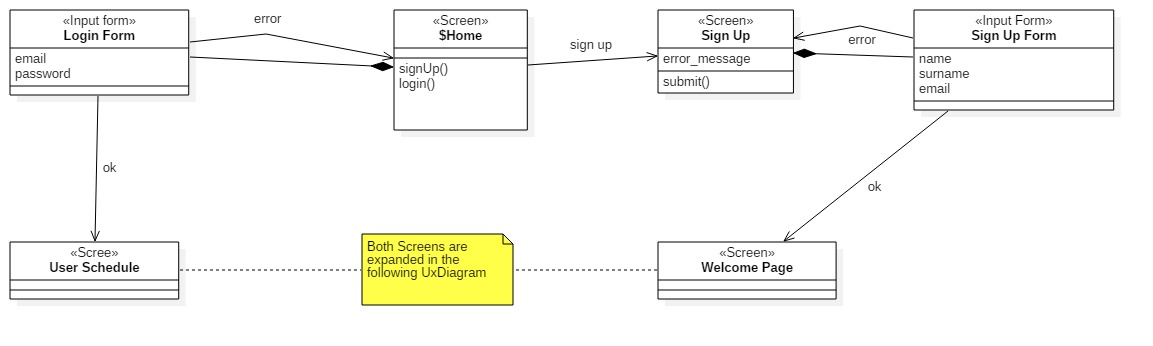
\includegraphics[width=0.9\paperwidth]{Images/UxPerson}}
		\caption{UX Diagram - Person UX}
	\end{figure}	
	\begin{figure}[H]	
		\centerline{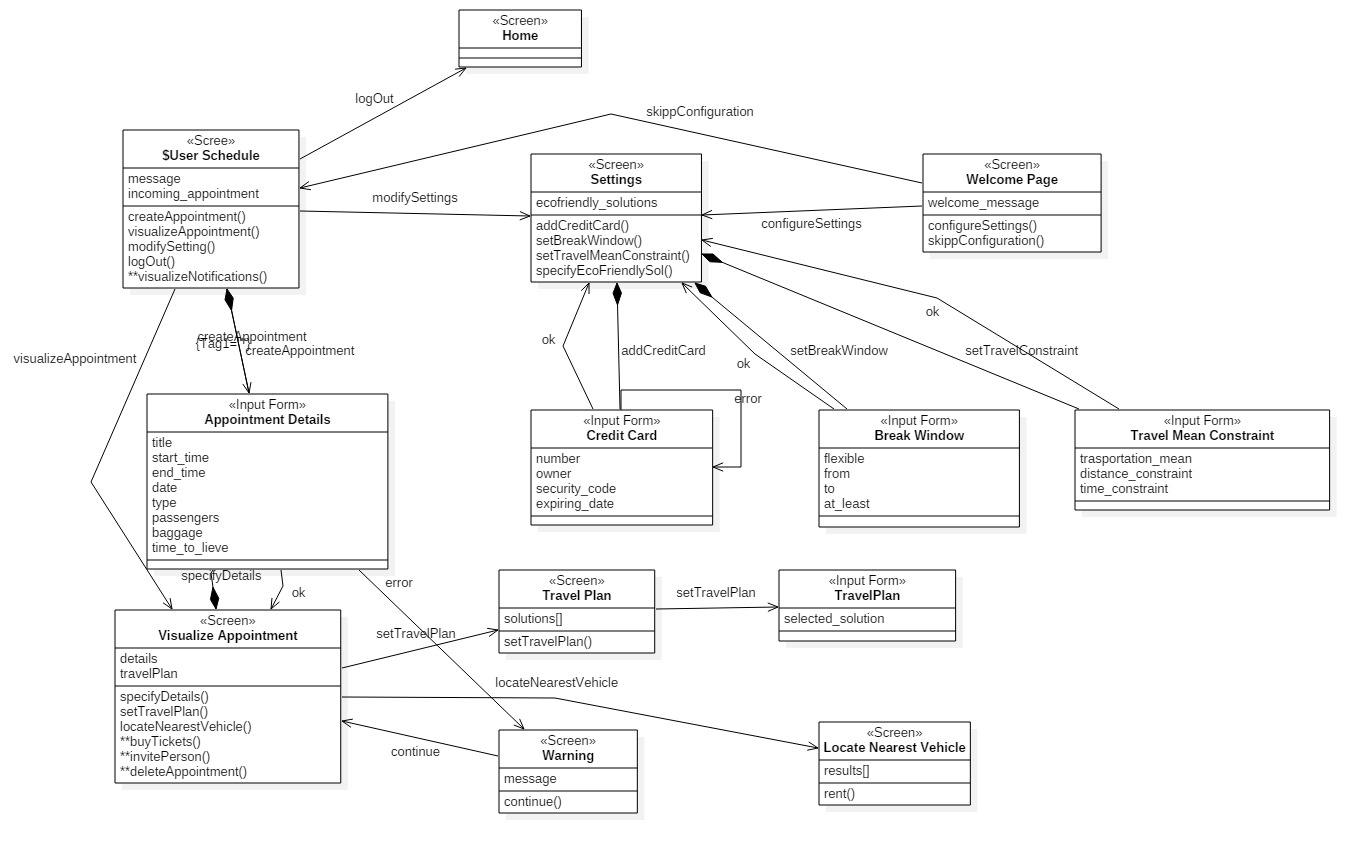
\includegraphics[width=0.9\paperwidth]{Images/UxUser}}
		\caption{UX Diagram - User UX}
	\end{figure}

\subsection{App Mockups}
Here we provide several mockups to highlight what we described in the UX Diagrams above. To logging in, a user has to insert his credentials in the Home Page. After that he is redirected to his Schedule from where he can access all the functionalities with no more than 3 clicks.

\begin{figure}[H]	
	\centerline{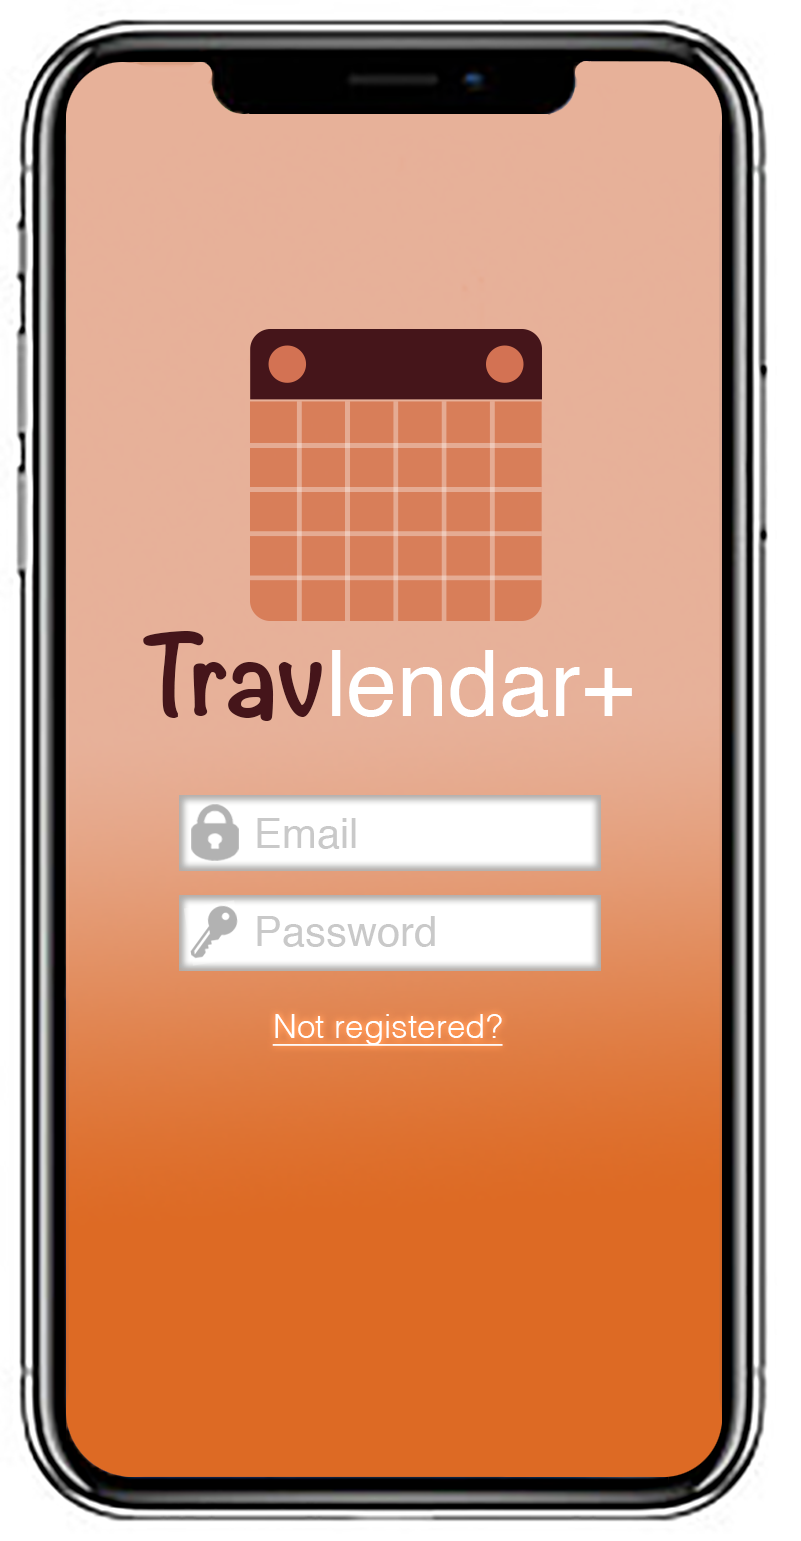
\includegraphics[width=0.3\paperwidth]{Images/Home}}
	\caption{Mockup - Home Page}
\end{figure}	
\begin{figure}[H]	
	\centerline{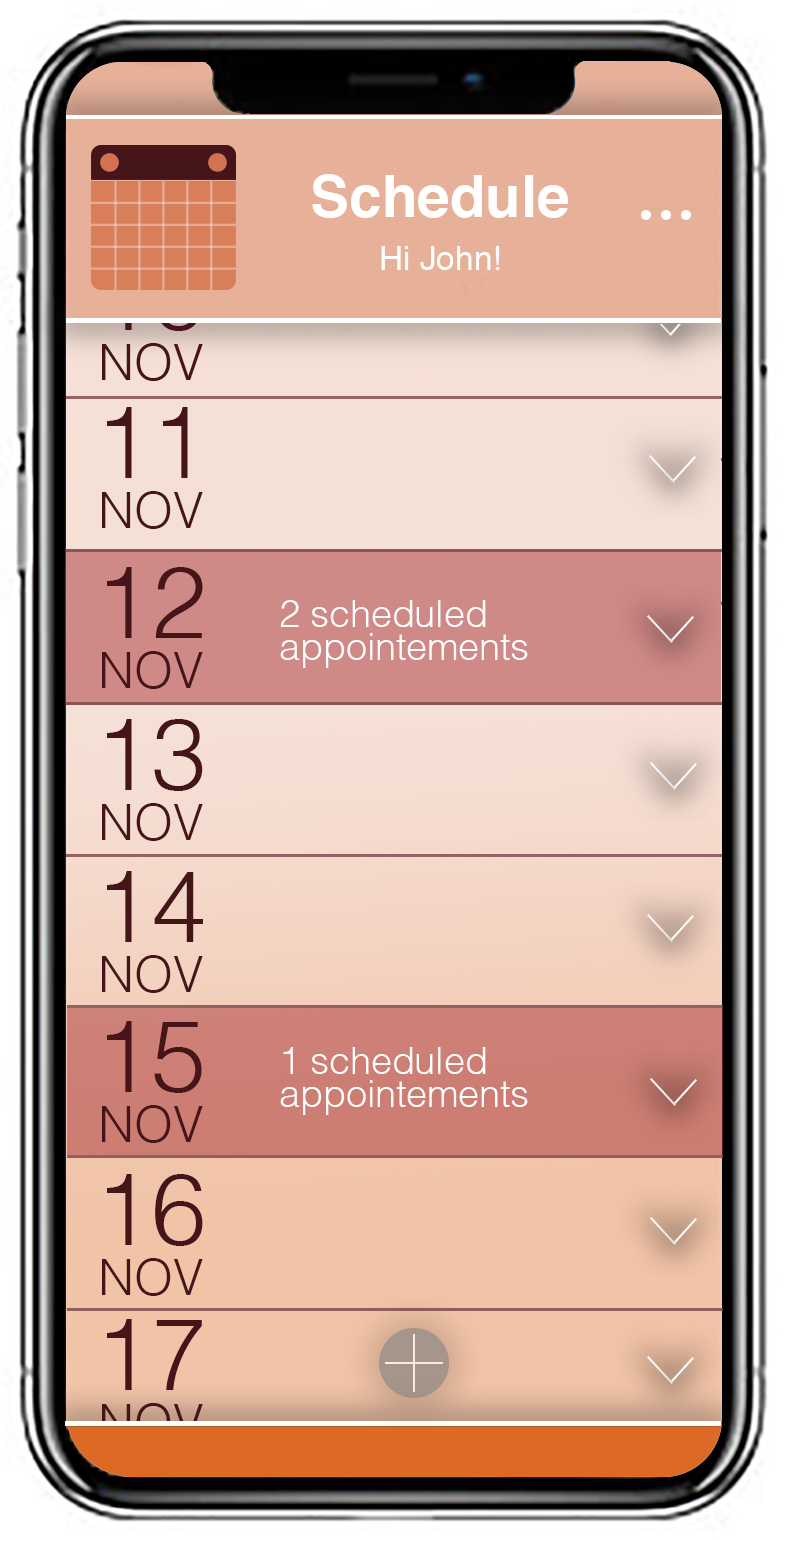
\includegraphics[width=0.3\paperwidth]{Images/UserSchedule}}
	\caption{Mockup - User Schedule}
\end{figure}
\begin{figure}[H]	
	\centerline{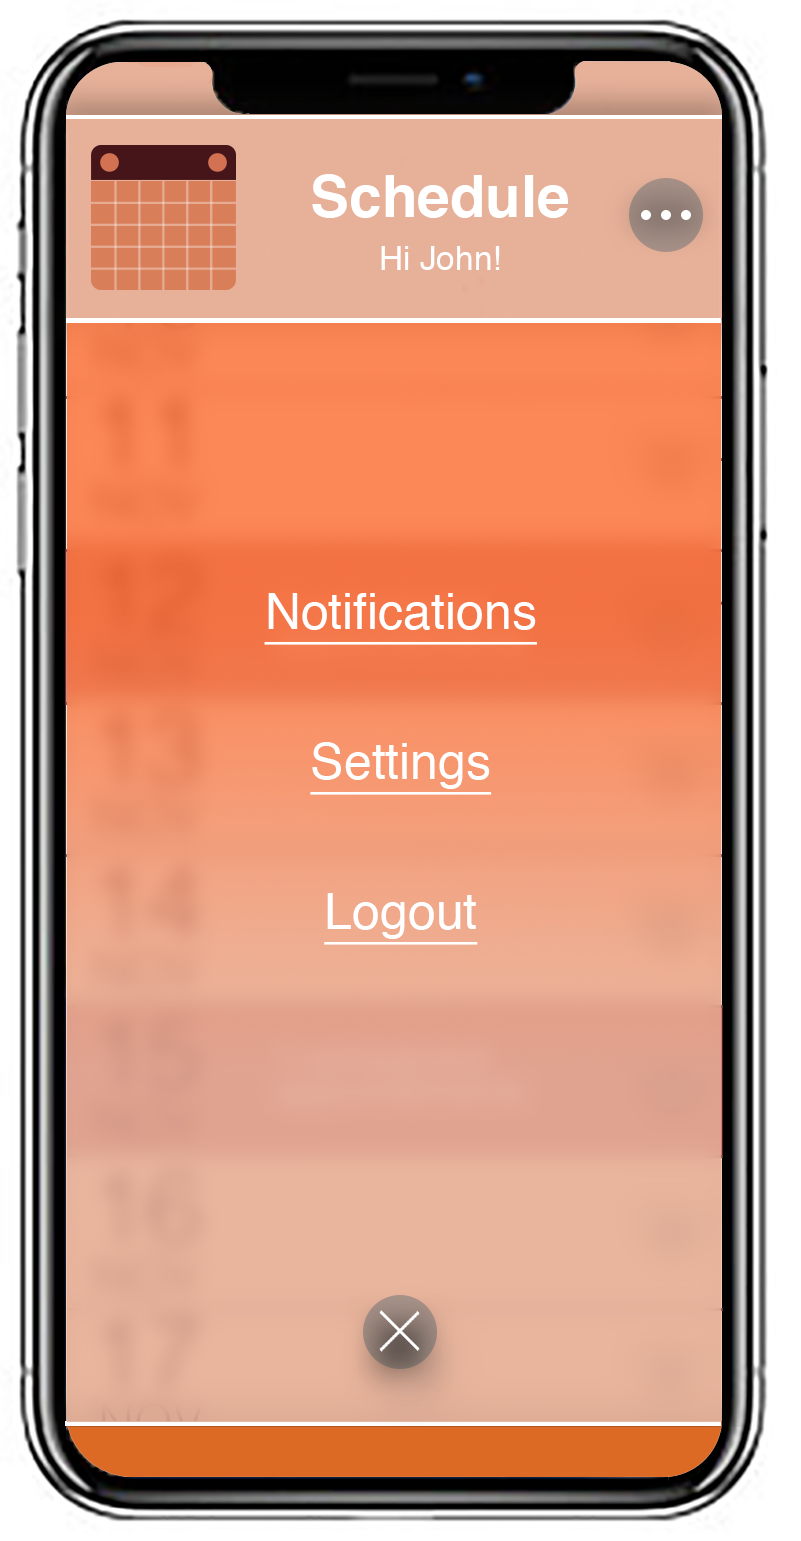
\includegraphics[width=0.3\paperwidth]{Images/Settings}}
	\caption{Mockup -Settings}
\end{figure}	
\begin{figure}[H]	
	\centerline{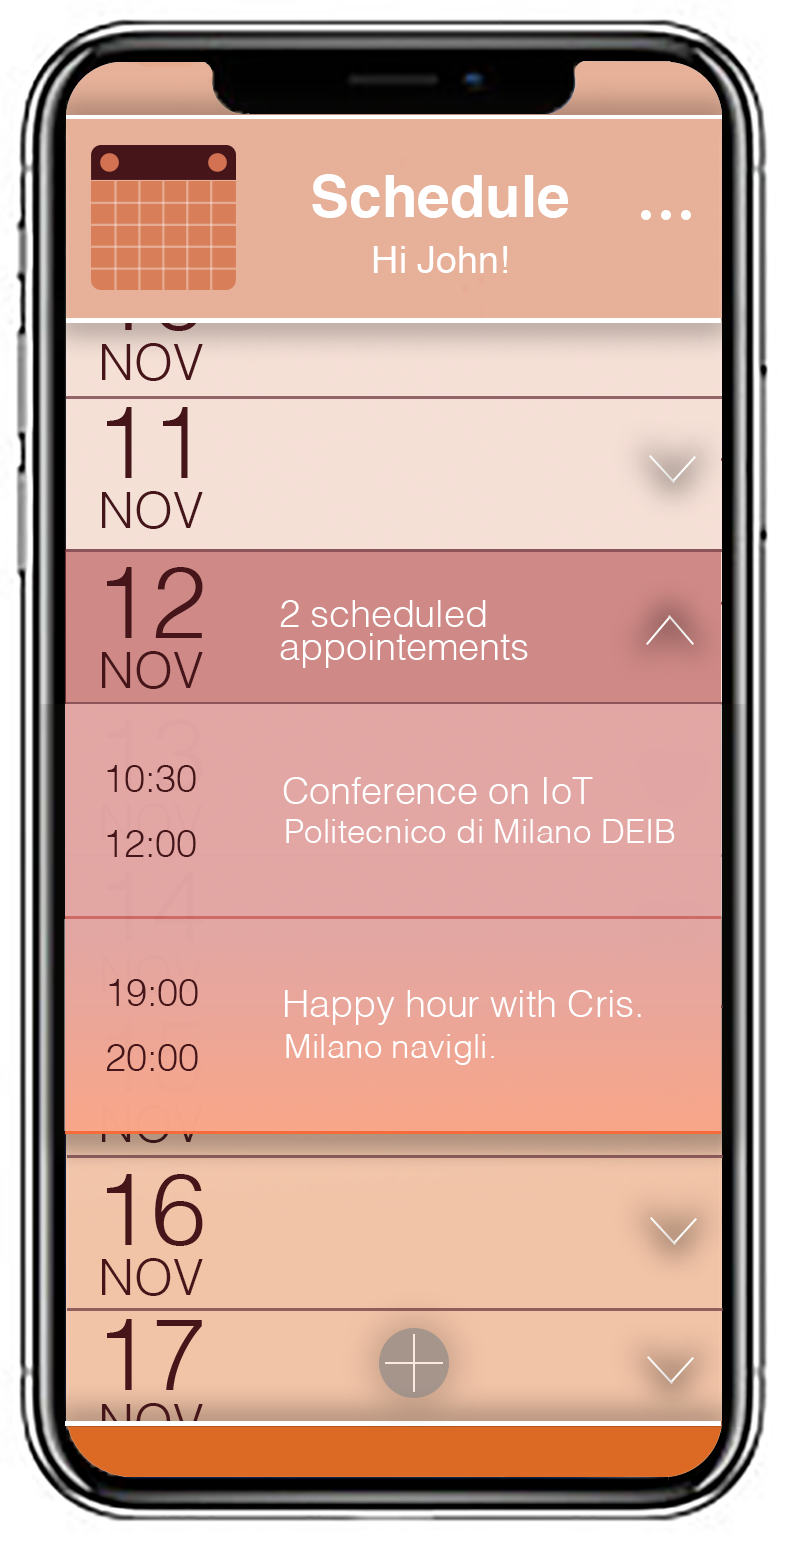
\includegraphics[width=0.3\paperwidth]{Images/DailySchedule}}
	\caption{Mockup - Daily Schedule}
\end{figure}
\begin{figure}[H]	
	\centerline{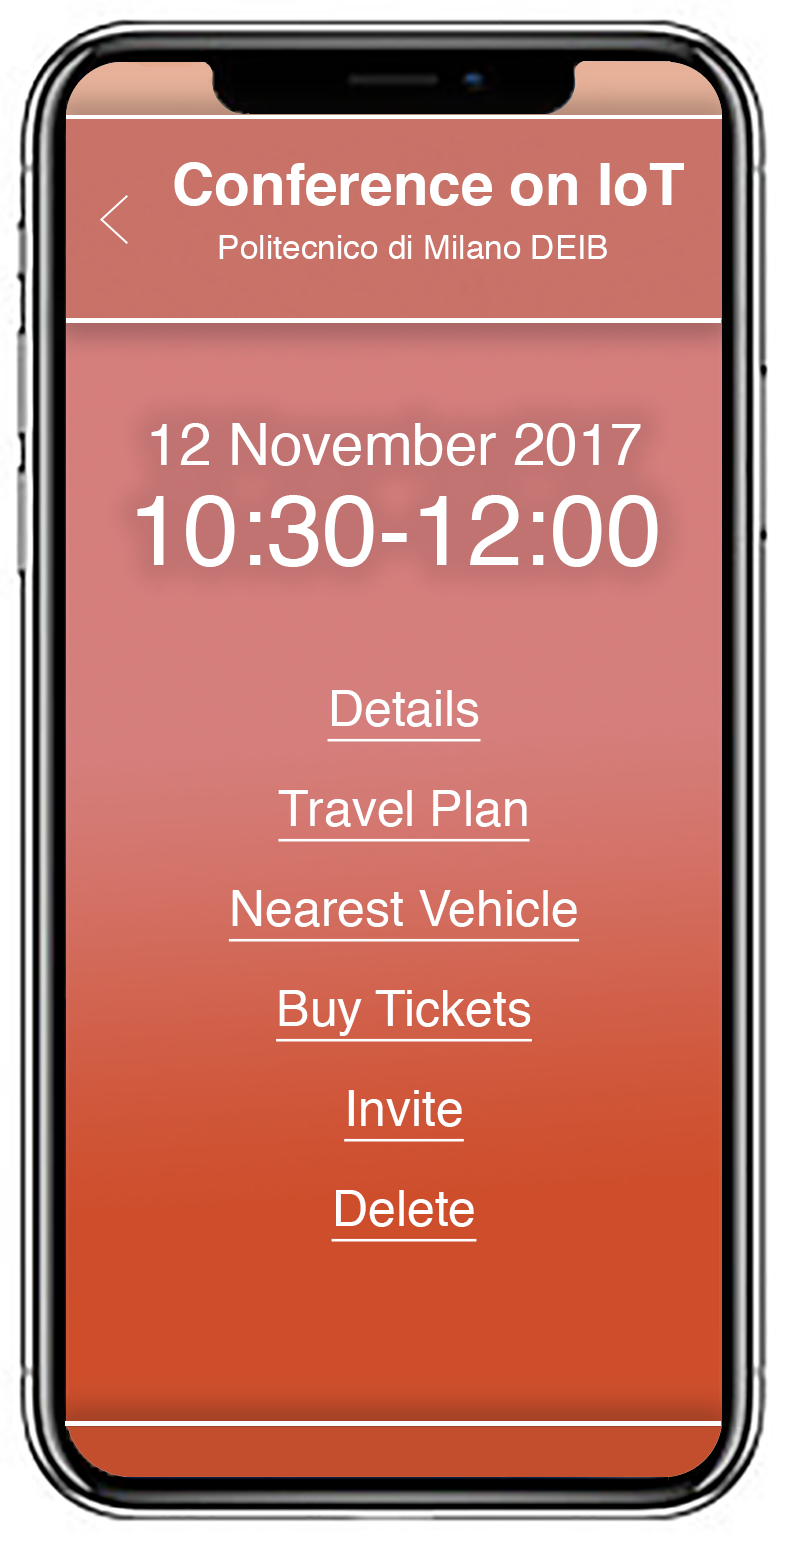
\includegraphics[width=0.3\paperwidth]{Images/VisualizeAppointment}}
	\caption{Mockup -Visualize Appointment}
\end{figure}	
\begin{figure}[H]	
	\centerline{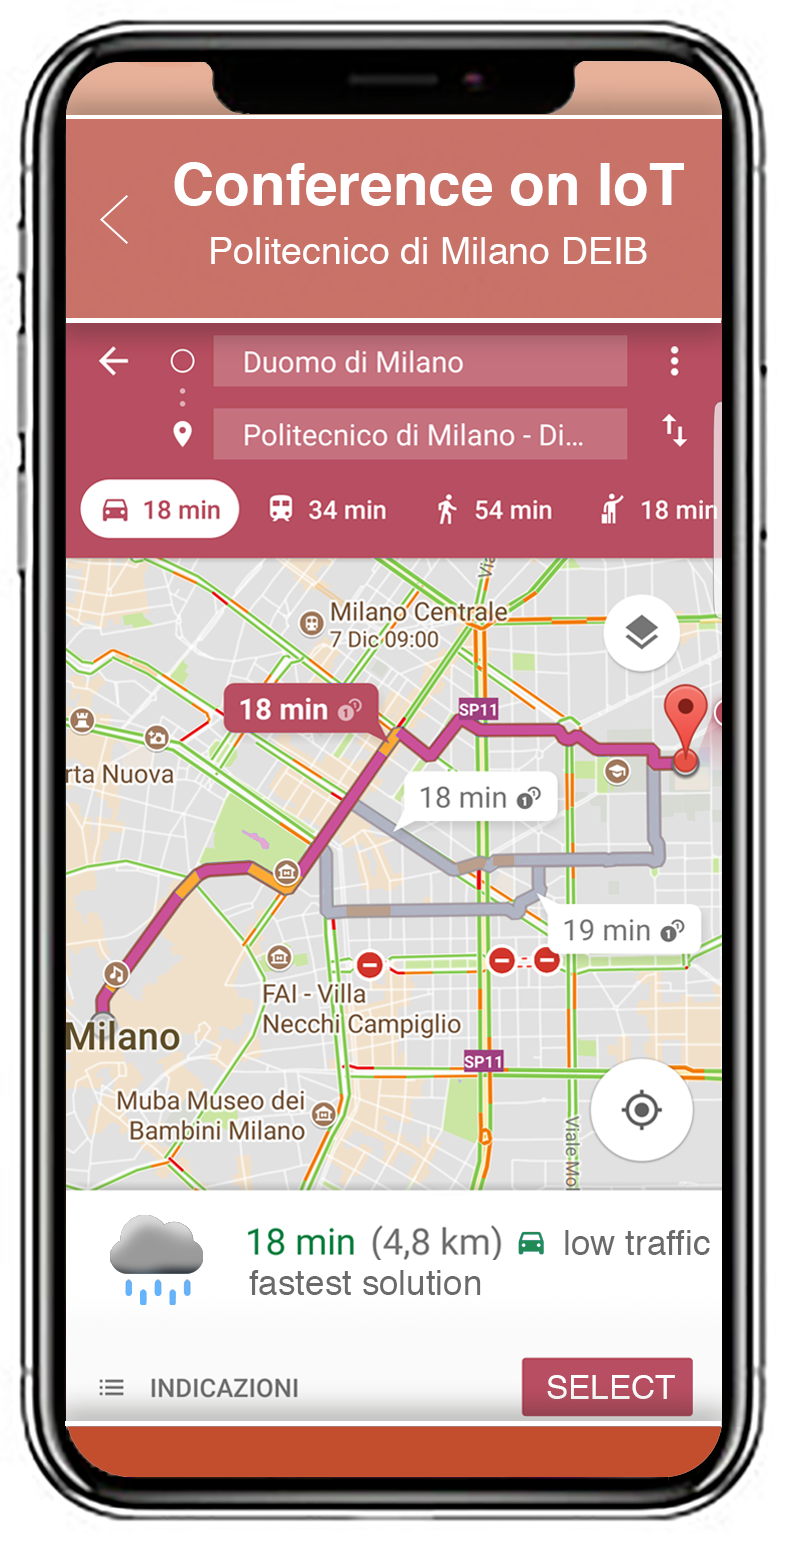
\includegraphics[width=0.3\paperwidth]{Images/SelectTravelPlan}}
	\caption{Mockup - Select TravelPlan}
\end{figure}
\begin{figure}[H]	
	\centerline{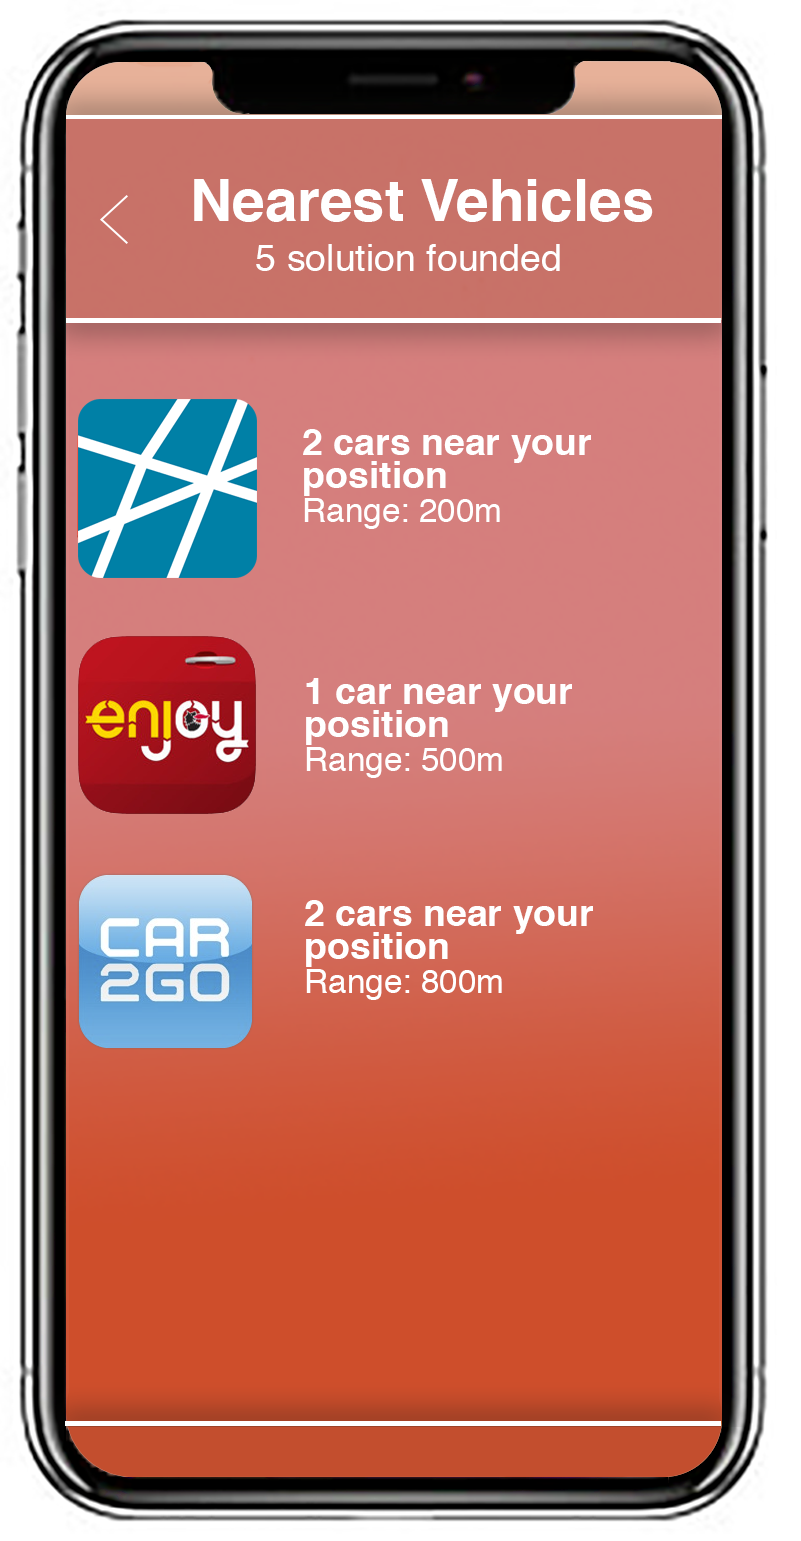
\includegraphics[width=0.3\paperwidth]{Images/LocateNearestVehicle}}
	\caption{Mockup - Locate Nearest Vehicle}
\end{figure}